

\subsection{Compilazione Singolo file}
Un file sorgente in \code{C++} ha come estensione \code{.cpp} il comando per compilare un file sorgente in \code{.cpp} è:
\newline
\lstinputlisting{Capitoli/Compilatore/Esempi/g++NoOtimaizer.txt}

\begin{itemize}
    \item \textbf{\textcolor{blue}{\code{g++}}} : Compilatore \textbf{GNU} (ne esistono anche altri)
    \item \textbf{\textcolor{blue}{flag \code{-o}}} : per rinominare il file eseguibile in uscita
    \item \textbf{\textcolor{blue}{\code{.cpp}}} : Estensione file sorgente \code{C++} \newline
\end{itemize}

Possiamo esprimere anche un livello ti ottimizzazione del codice:

\lstinputlisting{Capitoli/Compilatore/Esempi/g++Otimaizer.txt}
\begin{itemize}
    \item \textbf{\textcolor{blue}{\code{-O3}}} : L'opzione \code{-ON} con \code{N = 0,1,2,3} sono i livelli di ottimizzazione del codice
\end{itemize}

\subsection{Compilazione Multifile}
Posso \textbf{spezzare} il mio codice in più file sorgente: tutti i file verranno compilati in file oggetto con estensione "\code{.o}" e poi uniti fra di loro termite il \textbf{linker} nella fase di \textbf{linking}.
\newline\newline il comando per fare ciò è: 
\lstinputlisting{Capitoli/Compilatore/Esempi/g++FileO.txt}
\begin{itemize}
    \item \textbf{\textcolor{blue}{\code{g++}}} : Compilatore \textbf{GNU} (ne esistono anche altri)
    \item \textbf{\textcolor{blue}{flag \code{-c}}} : non produce l'eseguibile ma solo il file oggetto(file sorgente tradotto in linguaggio macchina)
    \item \textbf{\textcolor{blue}{flag \code{-o}}} : per rinominare il file oggetto (solo se vogliamo un nome diverso da sorgente)
    
    \item \textbf{\textcolor{blue}{\code{.cpp}}} : Estensione file sorgente \code{C++} \newline \newpage
\end{itemize}
 Per fare il \textbf{linking} abbiamo: 
\lstinputlisting{Capitoli/Compilatore/Esempi/ComandoLinking.txt} 
quando il programma cresce di dimensione conviene ricompilare solo i files modificati per velocizzare il processo di compilazione del programma. e successivamente fare il \textbf{linking} fra i vari file oggetti. \newline

\subsection{ScriptBash o ScriptBatch}

Possiamo utilizzare dei script di shell (batch \code{.bat} o bash \code{.sh}): sono dei file che permettono di eseguire delle istruzioni automaticamente da schell. possiamo scrivere un programma che esegue correttamente tutti i passi per la compilazione de file che sono stati modificati  e creare un eseguitivo.\newline
\lstinputlisting{Capitoli/Compilatore/Esempi/FileBash.txt}

\subsection{Divisione in più file di un programma}
Un porgramma si deve dividere in più file per i \textbf{seguenti vantaggi:}
\begin{itemize}
    \item Più facilita nella lettura e comprensione del codice sia per noi che per i futuri programmatori che leggeranno il nostro codice
    \item Facilita nel lavoro di gruppo
    \item minor tempo di compilazione 
\end{itemize}

\subsection{Modularità}
\begin{itemize}
    \item \textbf{Struttura logica}: I componenti devono essere organizzati in modo che componenti che sono correlati siano nello stessi file. \newline
    quindi pezzi di codice(\textbf{componenti logici}) che sono molto correlati fra di loro andranno nello stesso file, altrimenti divisi.

    \item \textbf{Struttura fisica}: Come i vari pezzi di codice(\textbf{componenti logici}) sono divisi nei file. \newline
    questa suddivisone deve essere: 
    
    \begin{itemize} 
        \item \textcolor{blue}{Consistente}: Componenti \textbf{logici molto correlati} fra di loro devono  essere nello stesso file per rendere consistente il progetto. 
        \item \textcolor{blue}{Comprensibile} . Chiaro per chi lo legge.
        \item \textcolor{blue}{Flessibile} : Deve adattarsi a diverse esigenze. 
    \end{itemize}

    \item Molto importante anche dividere \textbf{l'interfacce} (es: firme delle funzioni)  dalla sua \textbf{L'implementazione} (es: Quello che fa la funzione) 
    
\end{itemize}

\subsection{Header File}
La direttiva al pre-processore \code{\#include nomefile.hpp} può avere più forme: \newline
\lstinputlisting{Capitoli/Compilatore/Esempi/HeaderFile.txt}
Nel \textbf{HeaderFile} vanno solo le dichiarazioni di funzioni, delle macro per il pre-processroe o struct.
più generalmente vanno solo la dichiarazione dei vari elementi.

\subsubsection{Inclusione Multipla}
Può accadere avvolte che uno stesso file \code{.hpp} venga incluso piu volte in file diversi.
facciamo un esempio: 
\begin{itemize}
    \item Abbiamo un file sorgente \code{test.hpp}
    \item abbiamo un secondo file \code{main.cpp}
\end{itemize}
Per ipotesi abbiamo incluso un file di nome \code{test.hpp} in tutti e due file.\newline
\begin{center}
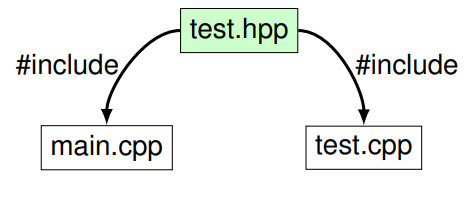
\includegraphics[scale = 0.6]{Capitoli/Compilatore/Esempi/esempioMultiplaInc.png}
\end{center}
\textbf{Come possiamo risolvere?} Basterà inserire nel file Header un \textbf{"flag"} che ci indichi se quel file è stato già inserito o meno.
\lstinputlisting{Capitoli/Compilatore/Esempi/testhppflag.txt}
quando viene incluso il file \code{test.hpp} prima di essere inserito nel file controllerà se \code{TEST\_HPP} non sia già stata dichiarata, nel caso in cui lo fosse non sarà incluso nulla.

\subsubsection{Sudivisone File Haeder File}
\begin{itemize}
 \item gli Header contiene \textbf{l'interfaccia} di tutto il contenuto del file sorgente corrispondente 
 \item Ogni file sorgente contiene un \code{\#include} per l’header
    corrispondente e poi eventuali altri header per tutto ciò che
    utilizza e la cui implementazione è data in altri file
 \item creare un file header \code{.hpp} per ogni file sorgente \code{.cpp}
\end{itemize}


\subsection{Fasi compilazione}

In questa fase abbiamo 4 fasi che restituiscono i seguenti file(Nome file "\code{primo.cpp}"):
\begin{itemize}
    \item \textbf{primo.i:} output Preprocessing
    \item \textbf{primo.s:} output fase di Compiling
    \item \textbf{primo.o:} output assembly
    \item \textbf{a.out:} output della fase di linking
\end{itemize}

\subsubsection{Preprocessing stage}
in questa fase succederà:
\begin{itemize}
    
    \item rimozione commenti
    \item saranno esegui le macro (es. \code{\#define}) , verranno sostituite al interno del programma 
    \item i file saranno inclusi attraverso \code{\#include}
    verranno inseriti le posizioni precisi dei file inclusi 
    esegue tutte le azioni precedute dal \code{\#}
\end{itemize}

\subsubsection{Compiling stage}
in questa fase viene creato il codice assembly. Ogni macchina ha la propria architettura e il proprio 
funzionamento. Per colpa di quest'ultima il codice assembly varia da processore a processore. Per 
questo ogni volta che il programma viene compilato sarà trasformato prima in assembly.

\newpage

\subsubsection{Assembly stage}
\begin{itemize}
    \item il \textbf{codice assembly} viene convertito in linguaggio macchina
    \item il file risultato è chiamato file oggetto
    \item \textbf{non risolve} chiamate a funzione.
    \item il file output non sarà visibile con normali tool di testo perché verranno codificati in \code{ASCII}
    \item il file oggetto \code{.o} può essere generato tramite il flag -c: \newline  \code{gcc -c primo.c} . questo comando farà tutti le fasi tranne il linking cosi non generando l'eseguibile.
\end{itemize}

\subsubsection{Linking stage}
    \begin{itemize}
        \item vengono risolte le \textbf{chiamate a funzione}. verranno uniti tutti i file oggetti fra di loro
        \item viene creato l’eseguibile
    \end{itemize}